%=========Background============================================

\section*{Background}

This game revisits the classic problem of the Hunter and the Monkey. The monkey is at a distance away from the hunter. The hunter aims at the monkey at some angle and at the time he shoots, the monkey falls down from a tree. The question is at what angles will it result in a hit.

The solution to this problem can be solved analytically by utilizing the equations of motions derived from Newton's Law:

\begin{align}
    \vec{x} &= \vec{x}_0 + \Vec{v}_0*t + \frac{1}{2} \vec{a}*t^2 \\
    \vec{v} &= \vec{v}_0 + \vec{a}*t
\end{align}

Another approach is utilizing the differential form of Newton's Law, 

\begin{equation}
    \frac{d^2 x}{dt^2} = \frac{\vec{F}}{m}
\end{equation}

and solving it numerically with the fourth order Runge-Kutta method. 

The Runge-Kutta method can be described as calculating the slope on a point an advancing a step of size $h$. Then use the previous result to calculate the slope at half the step. Then, repeat but now using the last result. Then again, use the last result to calculate the slope but now advance a whole step. Finally, use the information from all the steps to calculate your next value. This process is visually explained on Figure \ref{fig:rk4Example}.

\begin{figure}
    \centering
    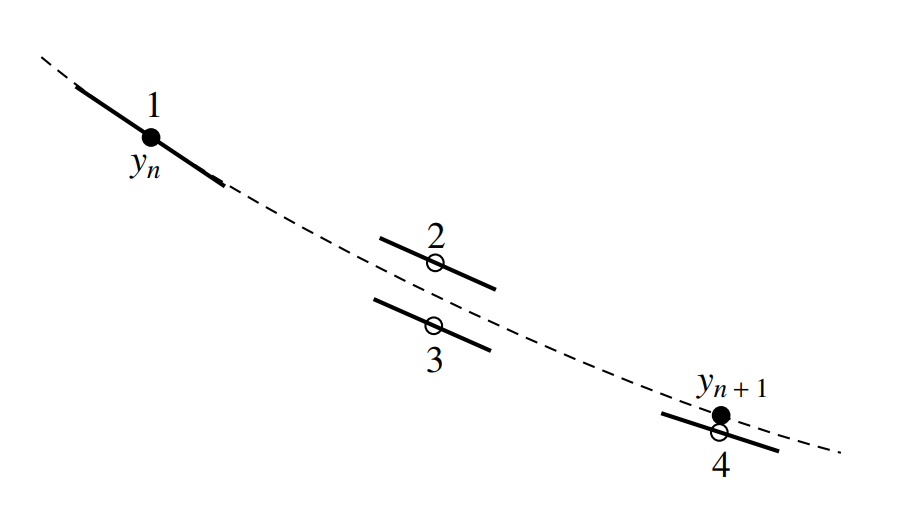
\includegraphics[width=\linewidth]{figures/rk4Example.png}
    \caption{Visual explanation of the fourth order Runge-Kutta method. \small{Source: Numerical Recipes 3rd Ed pg. 909}}
    \label{fig:rk4Example}
\end{figure}

Computationally, we need to program the following equation:

\begin{align*}
    k_1 &= hf(x_n, y_n)\\
    k_2 &= hf(x_n + \frac{1}{2}h, y_n + \frac{1}{2}k_1)\\
    k_3 &= hf(x_n + \frac{1}{2}h, y_n + \frac{1}{2}k_2)\\
    k_4 &= hf(x_n + h,y_n + k_3)\\
    y_{n=1} &= y_n + \frac{1}{6}k_1 + \frac{1}{3}k_2 + \frac{1}{3}k_3 + \frac{1}{6}k_4
\end{align*}


%=========The Game============================================

\section*{The Game}
This homework was programmed to be a game where the user has the option of selecting between 3 different modes and choose the angle to aim at the monkey. The 3 different play modes are:

\begin{itemize}
    \item Gravity only. 
    
    The bullet and the monkey are only affected by the force of gravity.This is the simplest mode. 
    
    \item Add air resistance.
    
    The forces acting on the bullet are gravity and air drag while the monkey is only affected by gravity. 
    
    \item Add wind.
    
    The forces acting on the bullet are gravity, air resistance and wind. The direction of the wind and the magnitude of the wind are chosen from a uniformly random distribution.
\end{itemize}

All modes give the user the option to retry to shoot the monkey in case of a "Miss" keeping the same conditions of the monkey's position (horizontal distance and height) and wind's speed and direction. In case of a "Hit", the game ends.

The initial conditions given are the following:

\begin{itemize}
    \item Horizontal distance between golfer and monkey is \SI{2000\pm 100}{\m}
    \item Vertical distance \SI{60 \pm 20}{\m}
    \item Approximate an spherical bullet with radius \SI{7.2}{\mm}
    \item Bullet mass of \SI{0.007}{\kilo\gram}
    \item Initial bullet velocity is \SI{1100}{\m\per\sec}
    \item Monkey's hit area is a circle with radius of \SI{10}{\mm}
\end{itemize}

%=========Part1: Gravity Only ============================================

\section*{Mode: Gravity only}

First, we need to know what forces are acting on the bullet. In this case, the bullet only feel a force acting upon it a.k.a the gravity force in the downward direction. For this case, our sum of forces will be 
\begin{equation*}
    \Sigma F = F_gravity = m_bullet * \vec{a}
\end{equation*}
where $\vec{a}=[0,-g]$. The differential equation to be define is,
\begin{equation}
    \frac{d^2 x}{dt^2} = \frac{dv}{dt}= \frac{\vec{F}}{m} = \vec{a}
\end{equation}
where $\vec{a}$ is the acceleration of the bullet. Note that the acceleration is a constant and does not depend of time for this particular case. Since we are interested on the position of bullet, we need a second differential equation:
\begin{equation}
    \frac{dx}{dt} = v
    \label{eq:dxdt}
\end{equation}
Both of these equations need to be simultaneously solved. For this reason, the RK4 code is as follows,
\begin{lstlisting}[language=Python]
def rk4(func,told,uold,vold,vWind,h):
    midt=told+h/2
    tnew=told+h
    k1v=h*func(told,uold,vold,vWind)
    k1u=h*vold
    k2v=h*func(midt,uold,vold+k1v/2,vWind)
    k2u=h*(vold+k1v/2)
    k3v=h*func(midt,uold,vold+k2v/2,vWind)
    k3u=h*(vold+k2v/2)
    k4v=h*func(tnew,uold,vold+k3v,vWind)
    k4u=h*(vold+k3v)
    vnew=vold+k1v/6+k2v/3+k3v/3+k4v/6
    unew=uold+k1u/6+k2u/3+k3u/3+k4u/6
    return tnew,unew,vnew
\end{lstlisting}

Notice how there's no equation function for calculating the k's of the position. Since equation \ref{eq:dxdt} is so simple, it was incorporated within the code. Also, making it this way, helped me visualize how both of these interlaced RK4 interact with each other.

According to our initial conditions, the horizontal distance between the golfer and the monkey is variable as well as the height of the monkey. This was achieved by using np.random.uniform( minValue, maxValue). The minimum and maximum value is the negative and the positive of the uncertainty given. The horizontal distance is $\pm 100$ and for the height is $\pm 60$. 

Given that we have an uncertainty involved in the game, the optimal angle can be calculated from the minimums and maximums values our distances can be as well as using the small angle approximation. The small angle approximation tell us that for very small angles,
\begin{align*}
    \sin{\theta} &\approx \theta \\
    \cos{\theta} &\approx 1-\frac{\theta}{2}\\
    \tan{\theta} &\approx \theta
\end{align*}

We define the angle to be $0\deg$ in the direction from the hunter to the monkey and $90\deg$ immediately upwards. So the relation between the distances and the angle to aim is
$\tan{\theta}=\frac{height}{distance}$. The maximum and minimum angle are given by 
\begin{align*}
    \theta_{min} &\approx \frac{height_{min}}{distance_{max}} = \frac{40}{2100} = 0.019 = 1.091^\circ \\
    \theta_{max} &\approx \frac{height_{max}}{distance_{min}} = \frac{80}{1900} = 0.042 = 2.411^\circ
\end{align*}

Figure \ref{fig:diffAngles} shows three pairs of plot. Each pair is compose of a plot showing the trajectory in terms of x-position and y-position calculated from RK4 method and from the equations of motion, and a second plot showing the $residuals = \vec{x}_{RK4}-\vec{x}_{EM}$  where $\vec{x}_{RK4}$ is the position given by RK4 method and $\vec{x}_{EM}$ is the position given by the Equations of Motion (EM). The plot showing the trajectory barely shows a difference between RK4 method and EM but the residuals show a big difference mainly in the x position. This difference doesn't show any consistent shape at evaluating different angles, even when, the angle is very close to the actual hit angle. For this reason, I think it may be some computation error. A pending test could be to change from float32 to float64. The y position consistently shows a very almost zero difference which increases at longer times. This can be explained by the accumulation of errors that is adding up as more operations are been calculated. Nevertheless, the difference is small after $200000$ iterations which proves that RK4 is a good approximation.

\begin{figure}[ht]
    \centering
    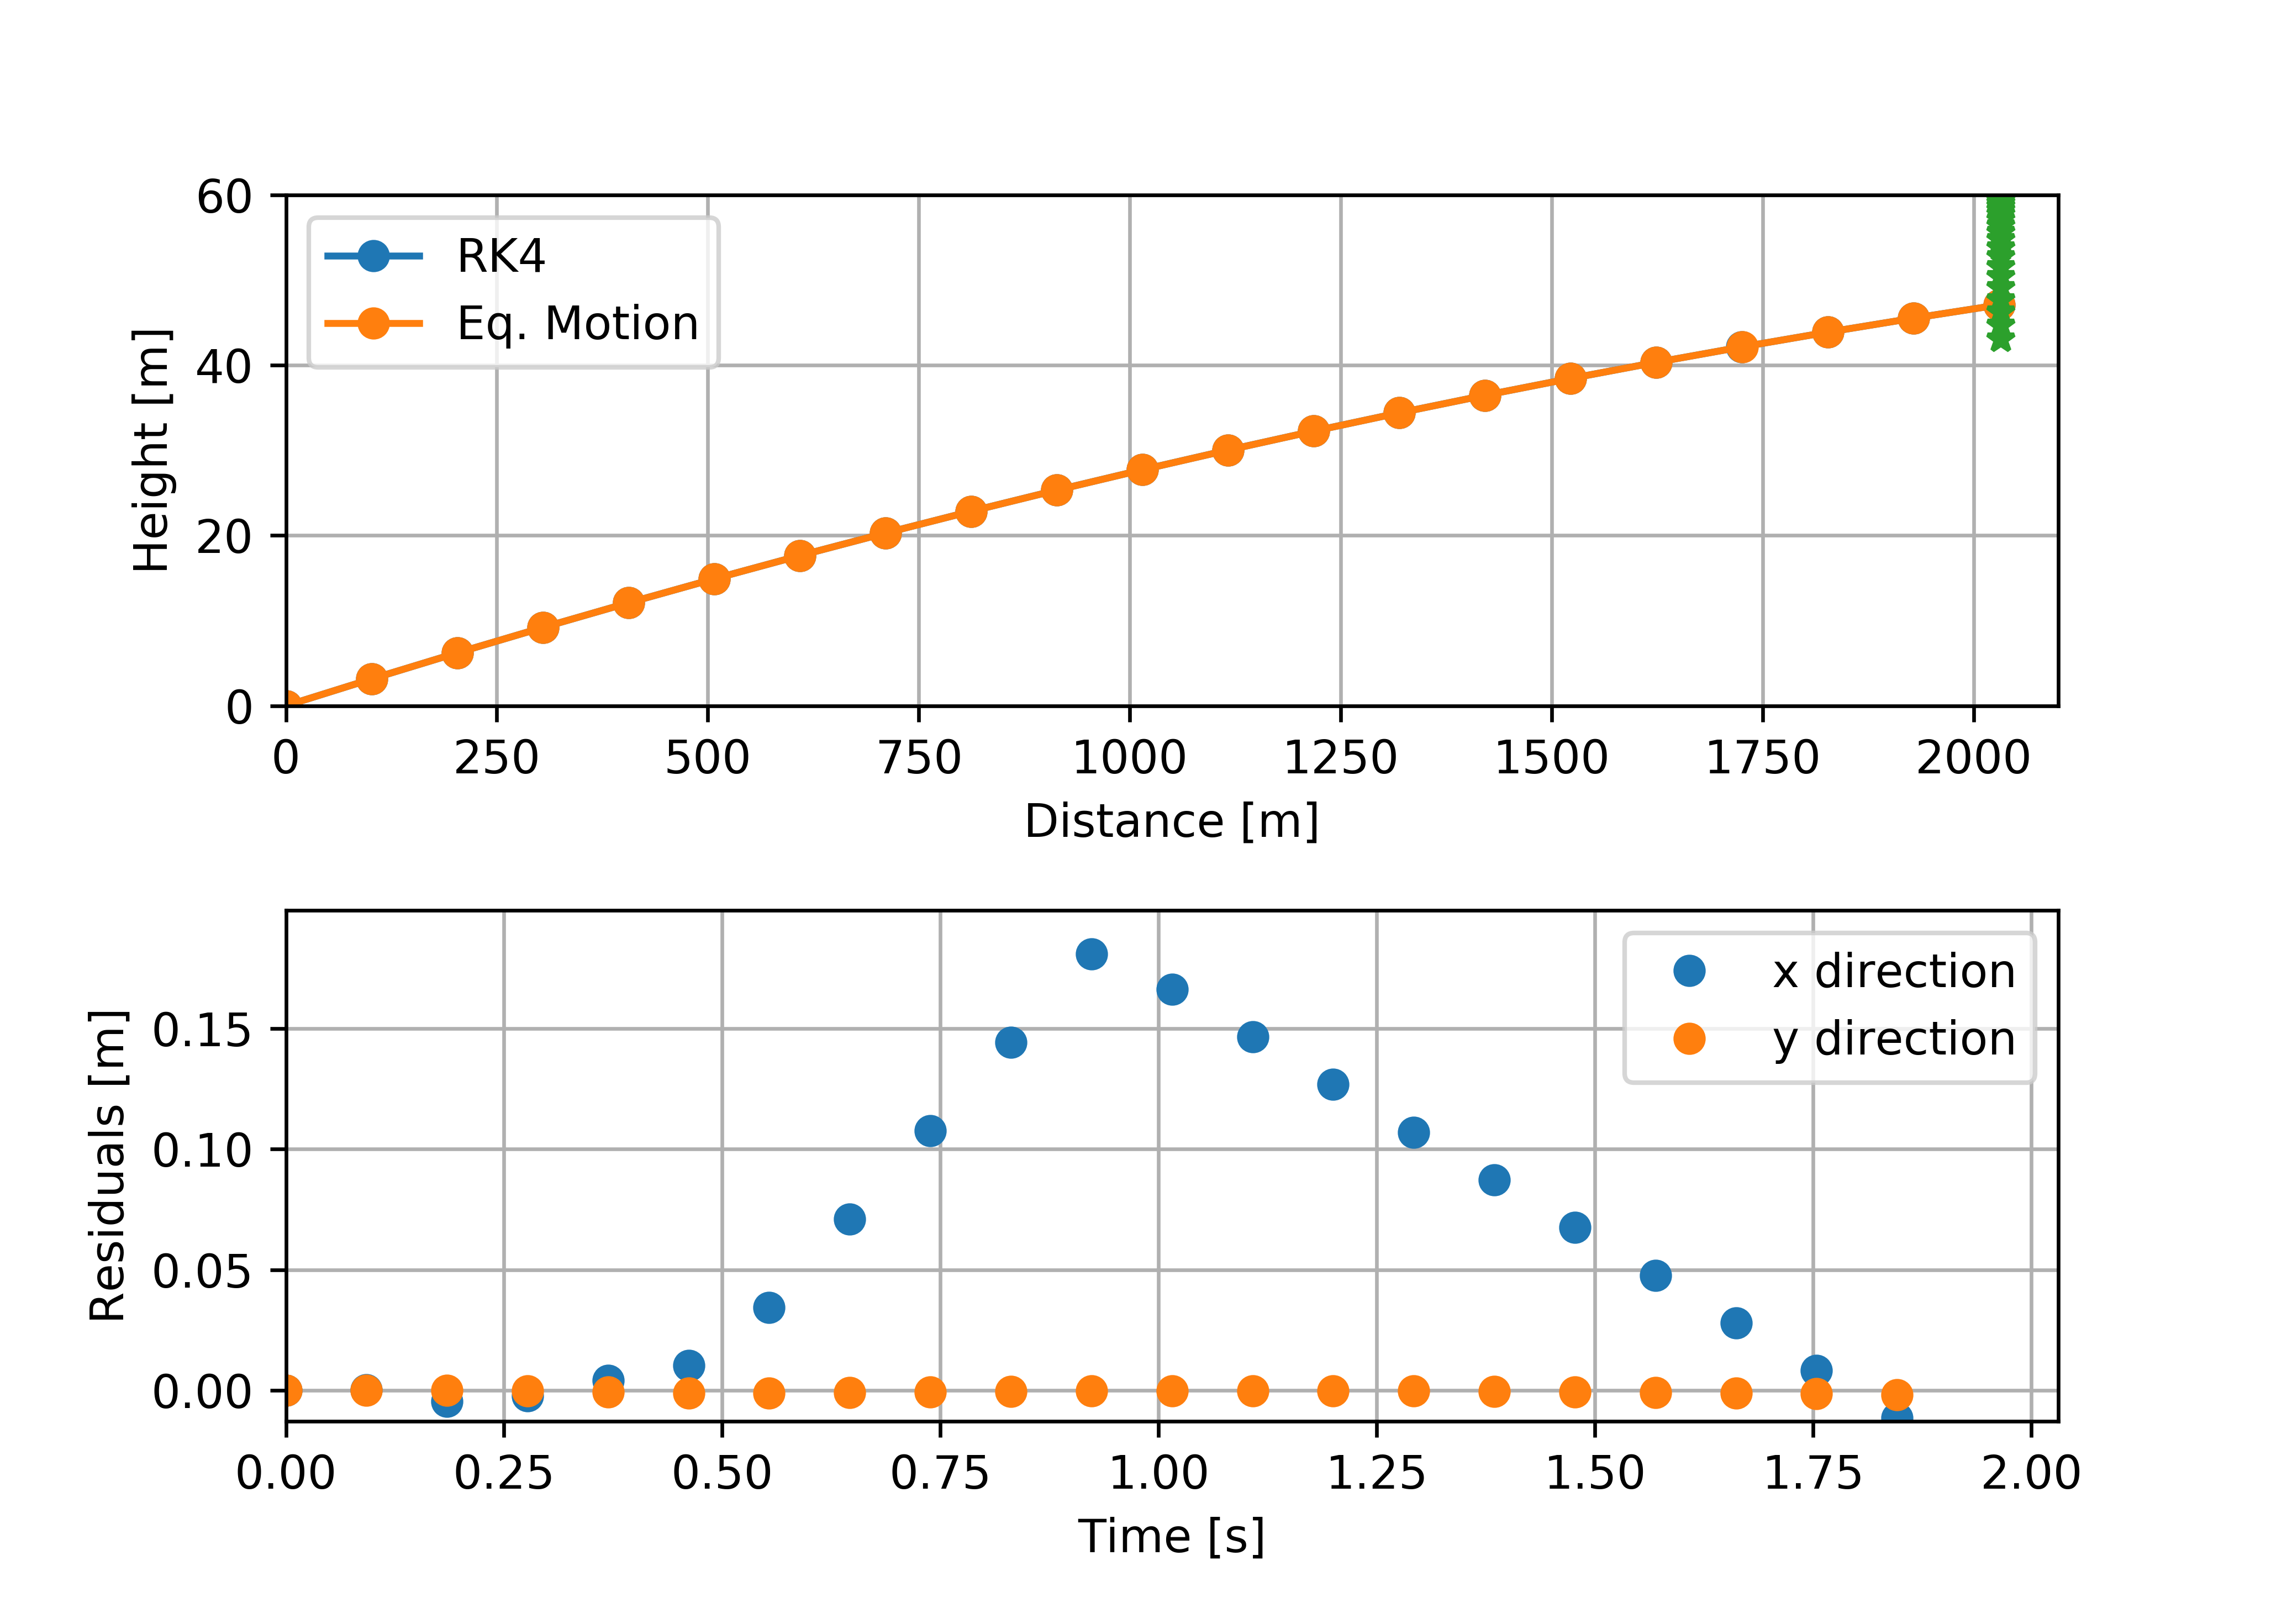
\includegraphics[width=.5\textwidth]{figures/a1-8x2031-6375y59-75881.png}
    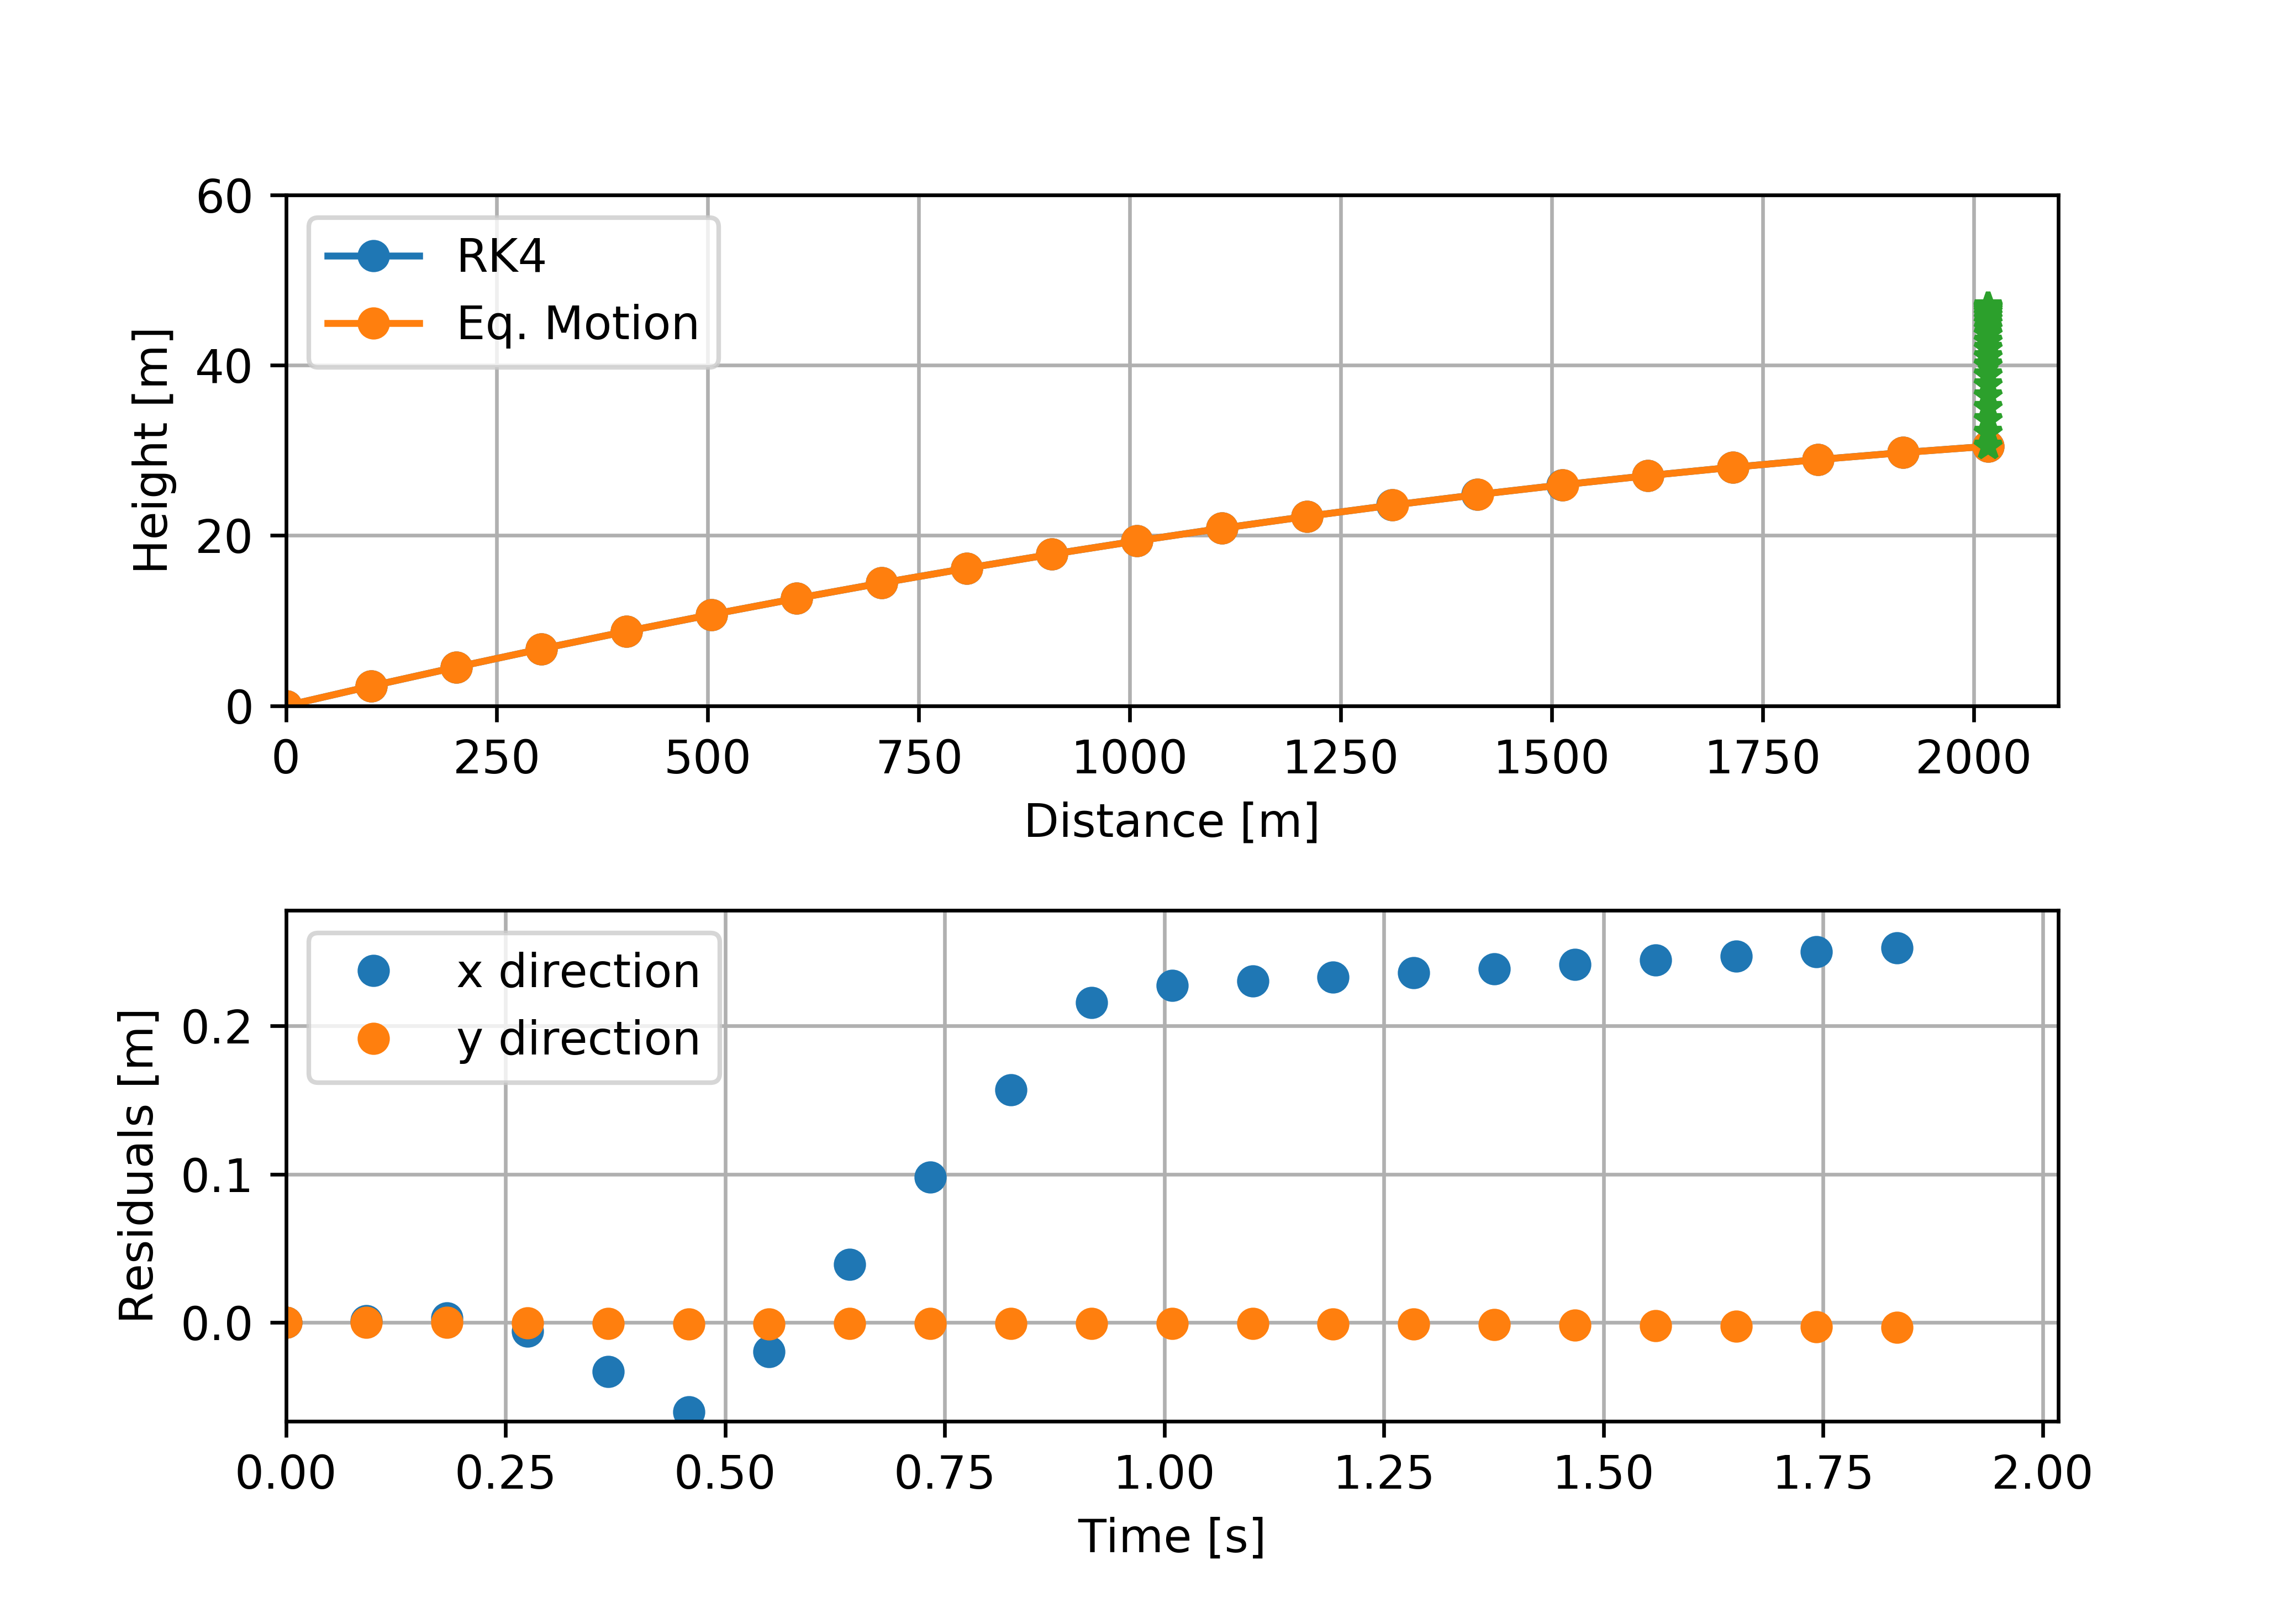
\includegraphics[width=.5\textwidth]{figures/a1-334x2017-1671y46-94758.png}
    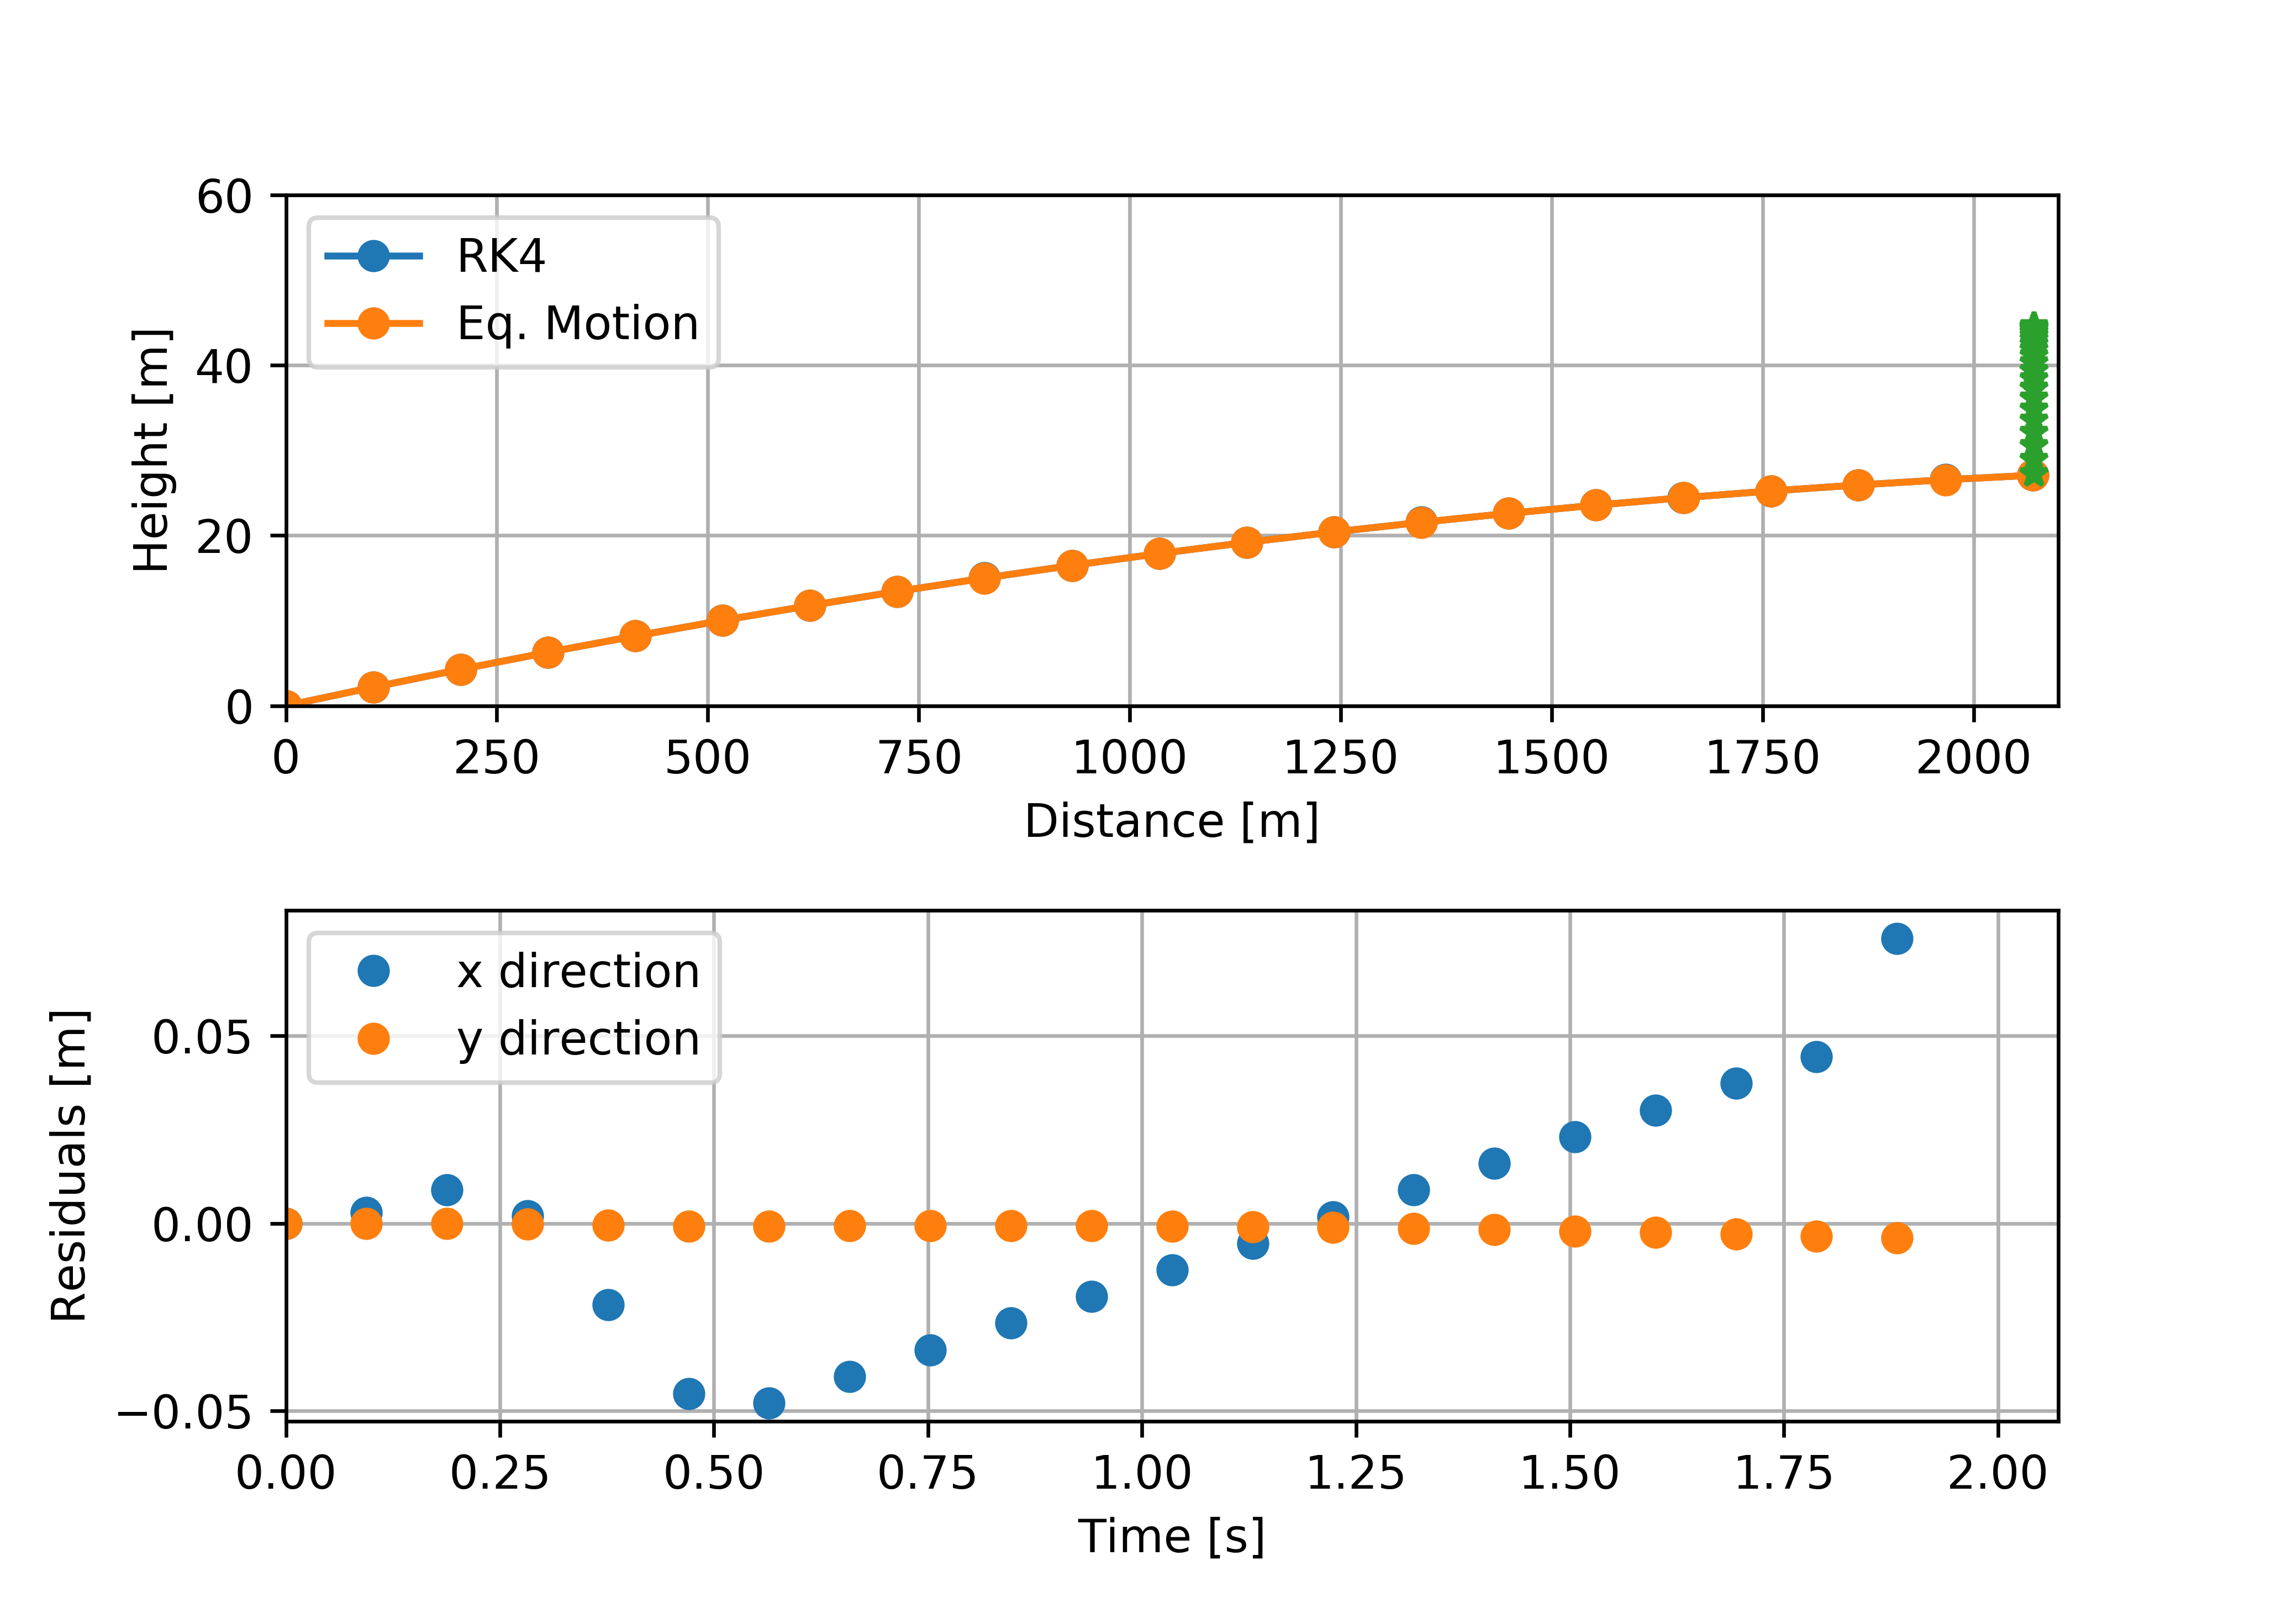
\includegraphics[width=.5\textwidth]{figures/a1-23x2071-4148y44-610104.png}
    \caption{Pairs of plots showing the trajectory followed by the golf ball using RK4 method and equations of motion as well as their residuals in x and y direction. 
    Top: Angle of \ang{1.8}, distance of \SI{2031.64}{\m} and height of \SI{59.76}{\m}. Middle: Angle of \ang{1.33}, distance of \SI{2017.17}{\m} and height of \SI{46.95}{\m}. Bottom: Angle of \ang{1.23}, distance of \SI{2071.41}{\m} and height of \SI{44.61}{\m}.}
    \label{fig:diffAngles}
\end{figure}{}

\begin{figure}[ht]
    \centering
    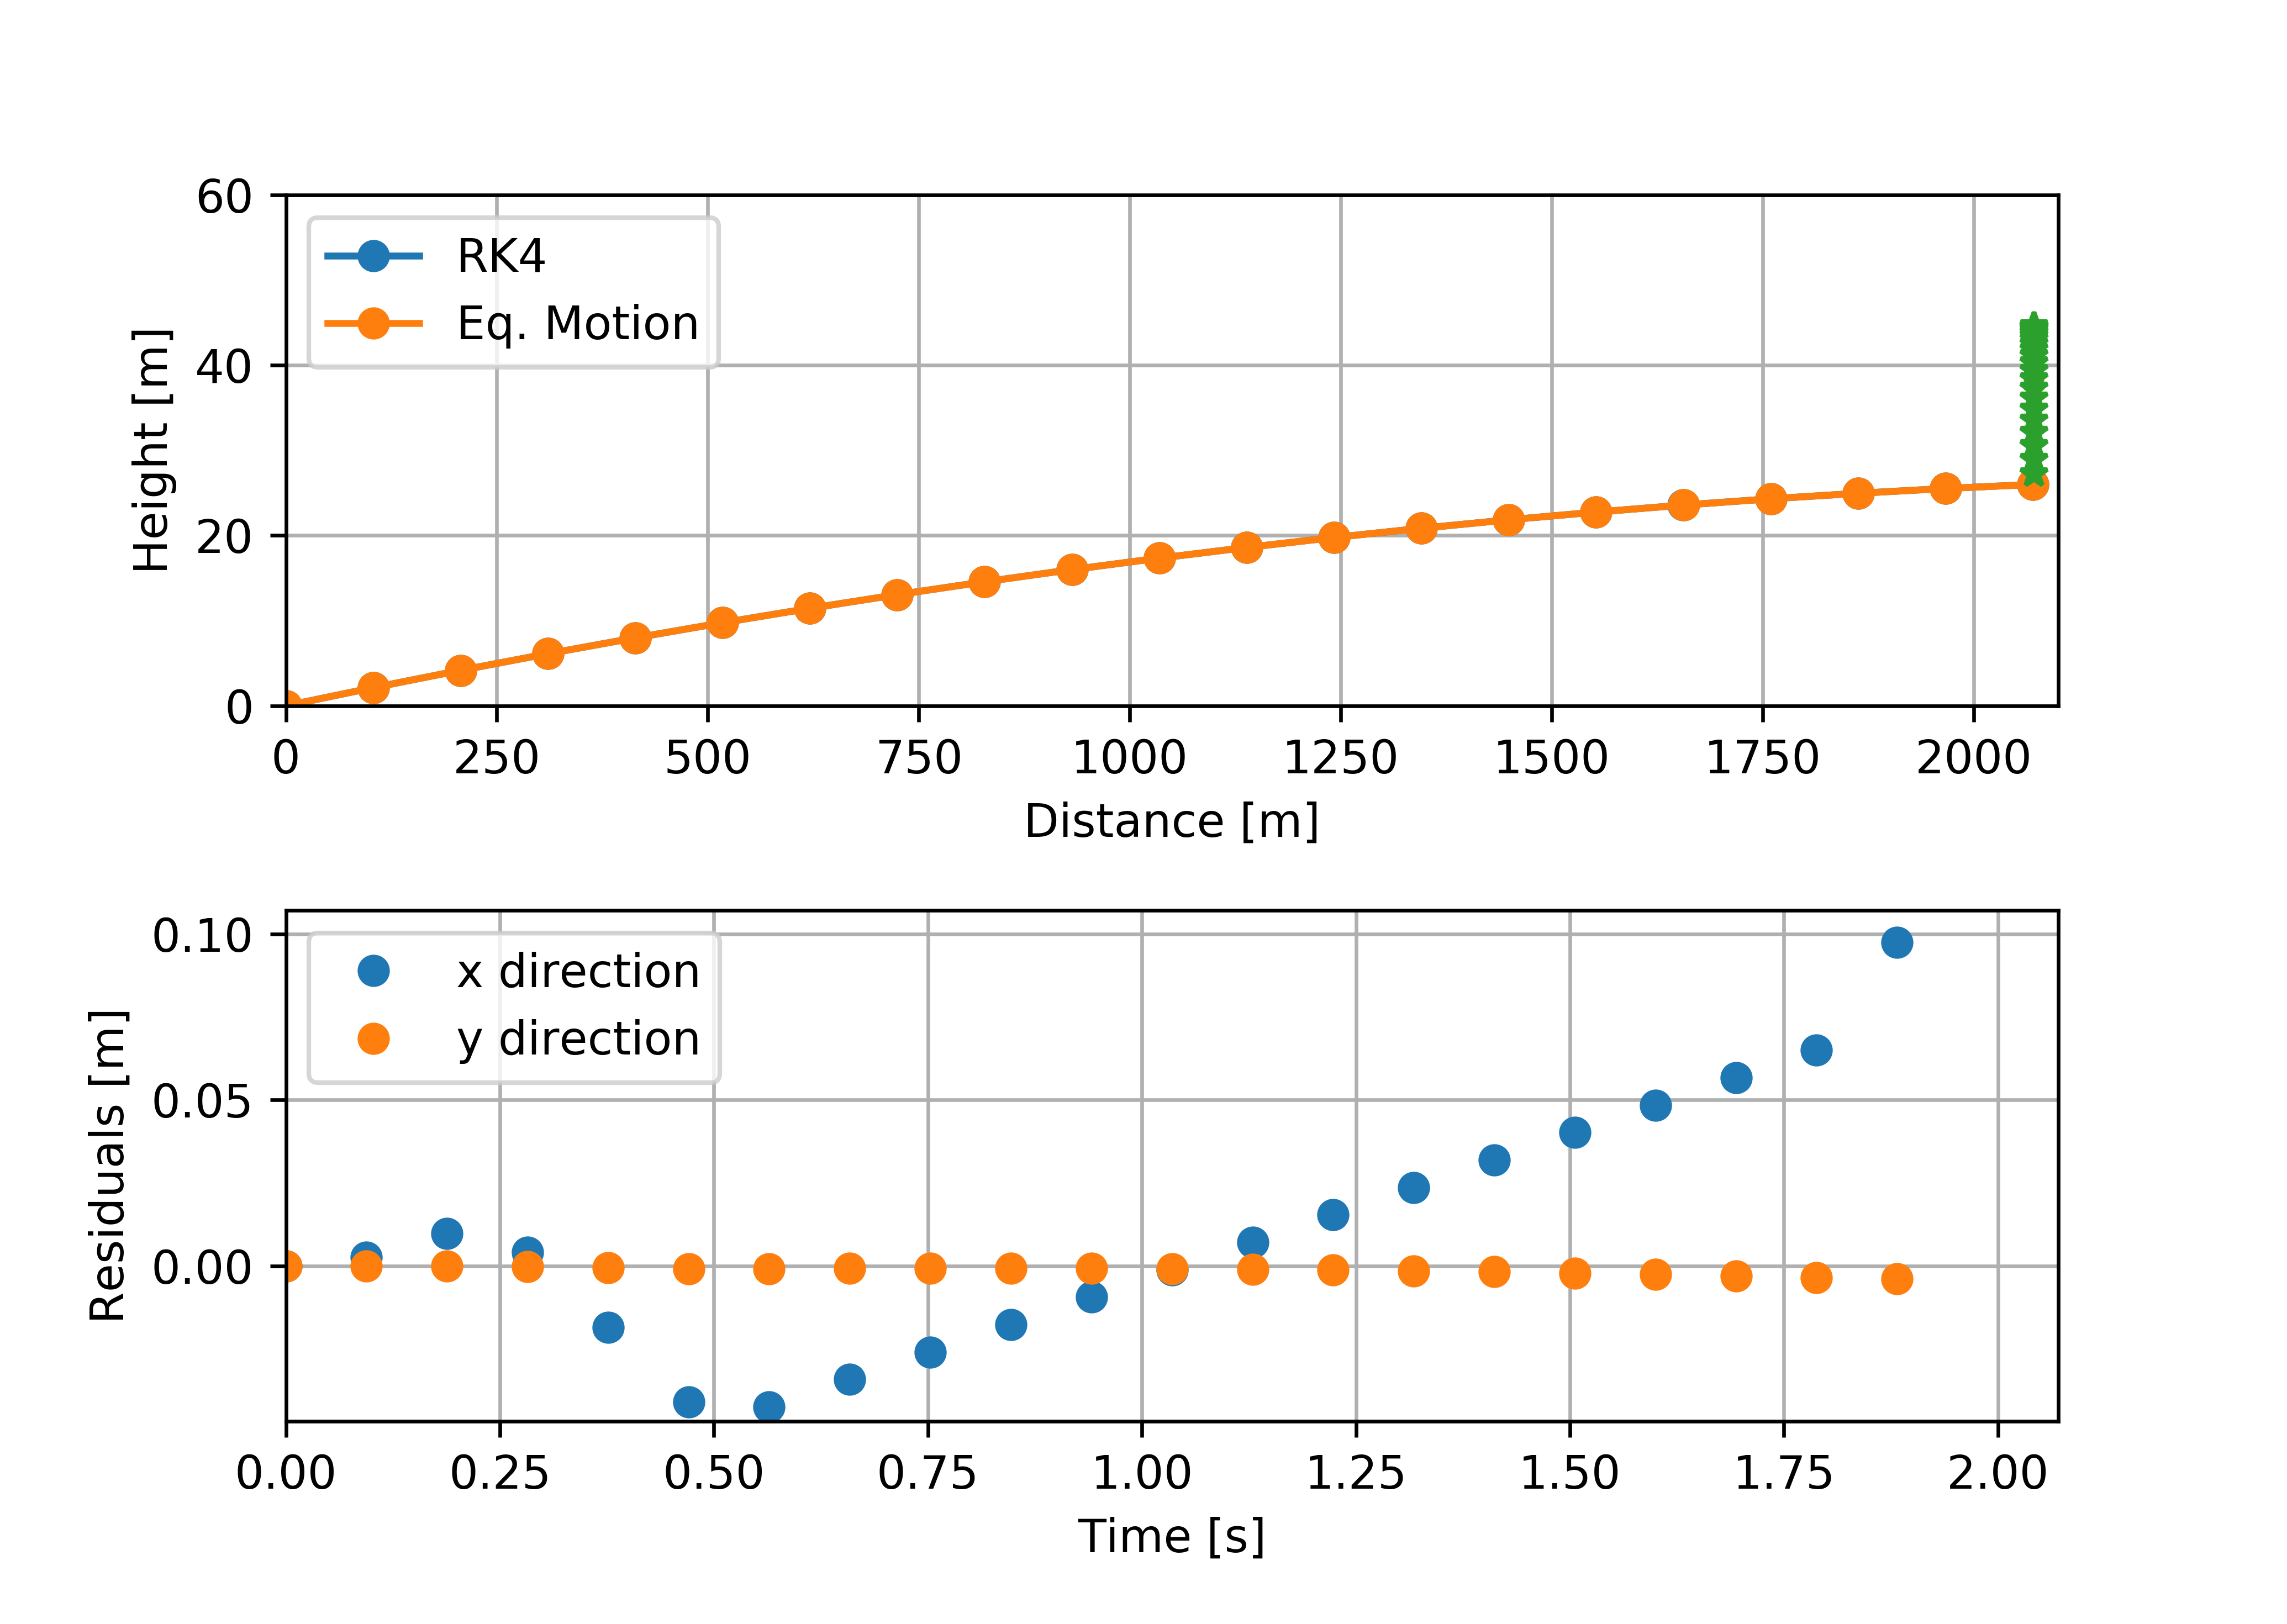
\includegraphics[width=.49\textwidth]{figures/a1-2x2071-4148y44-610104.png}
    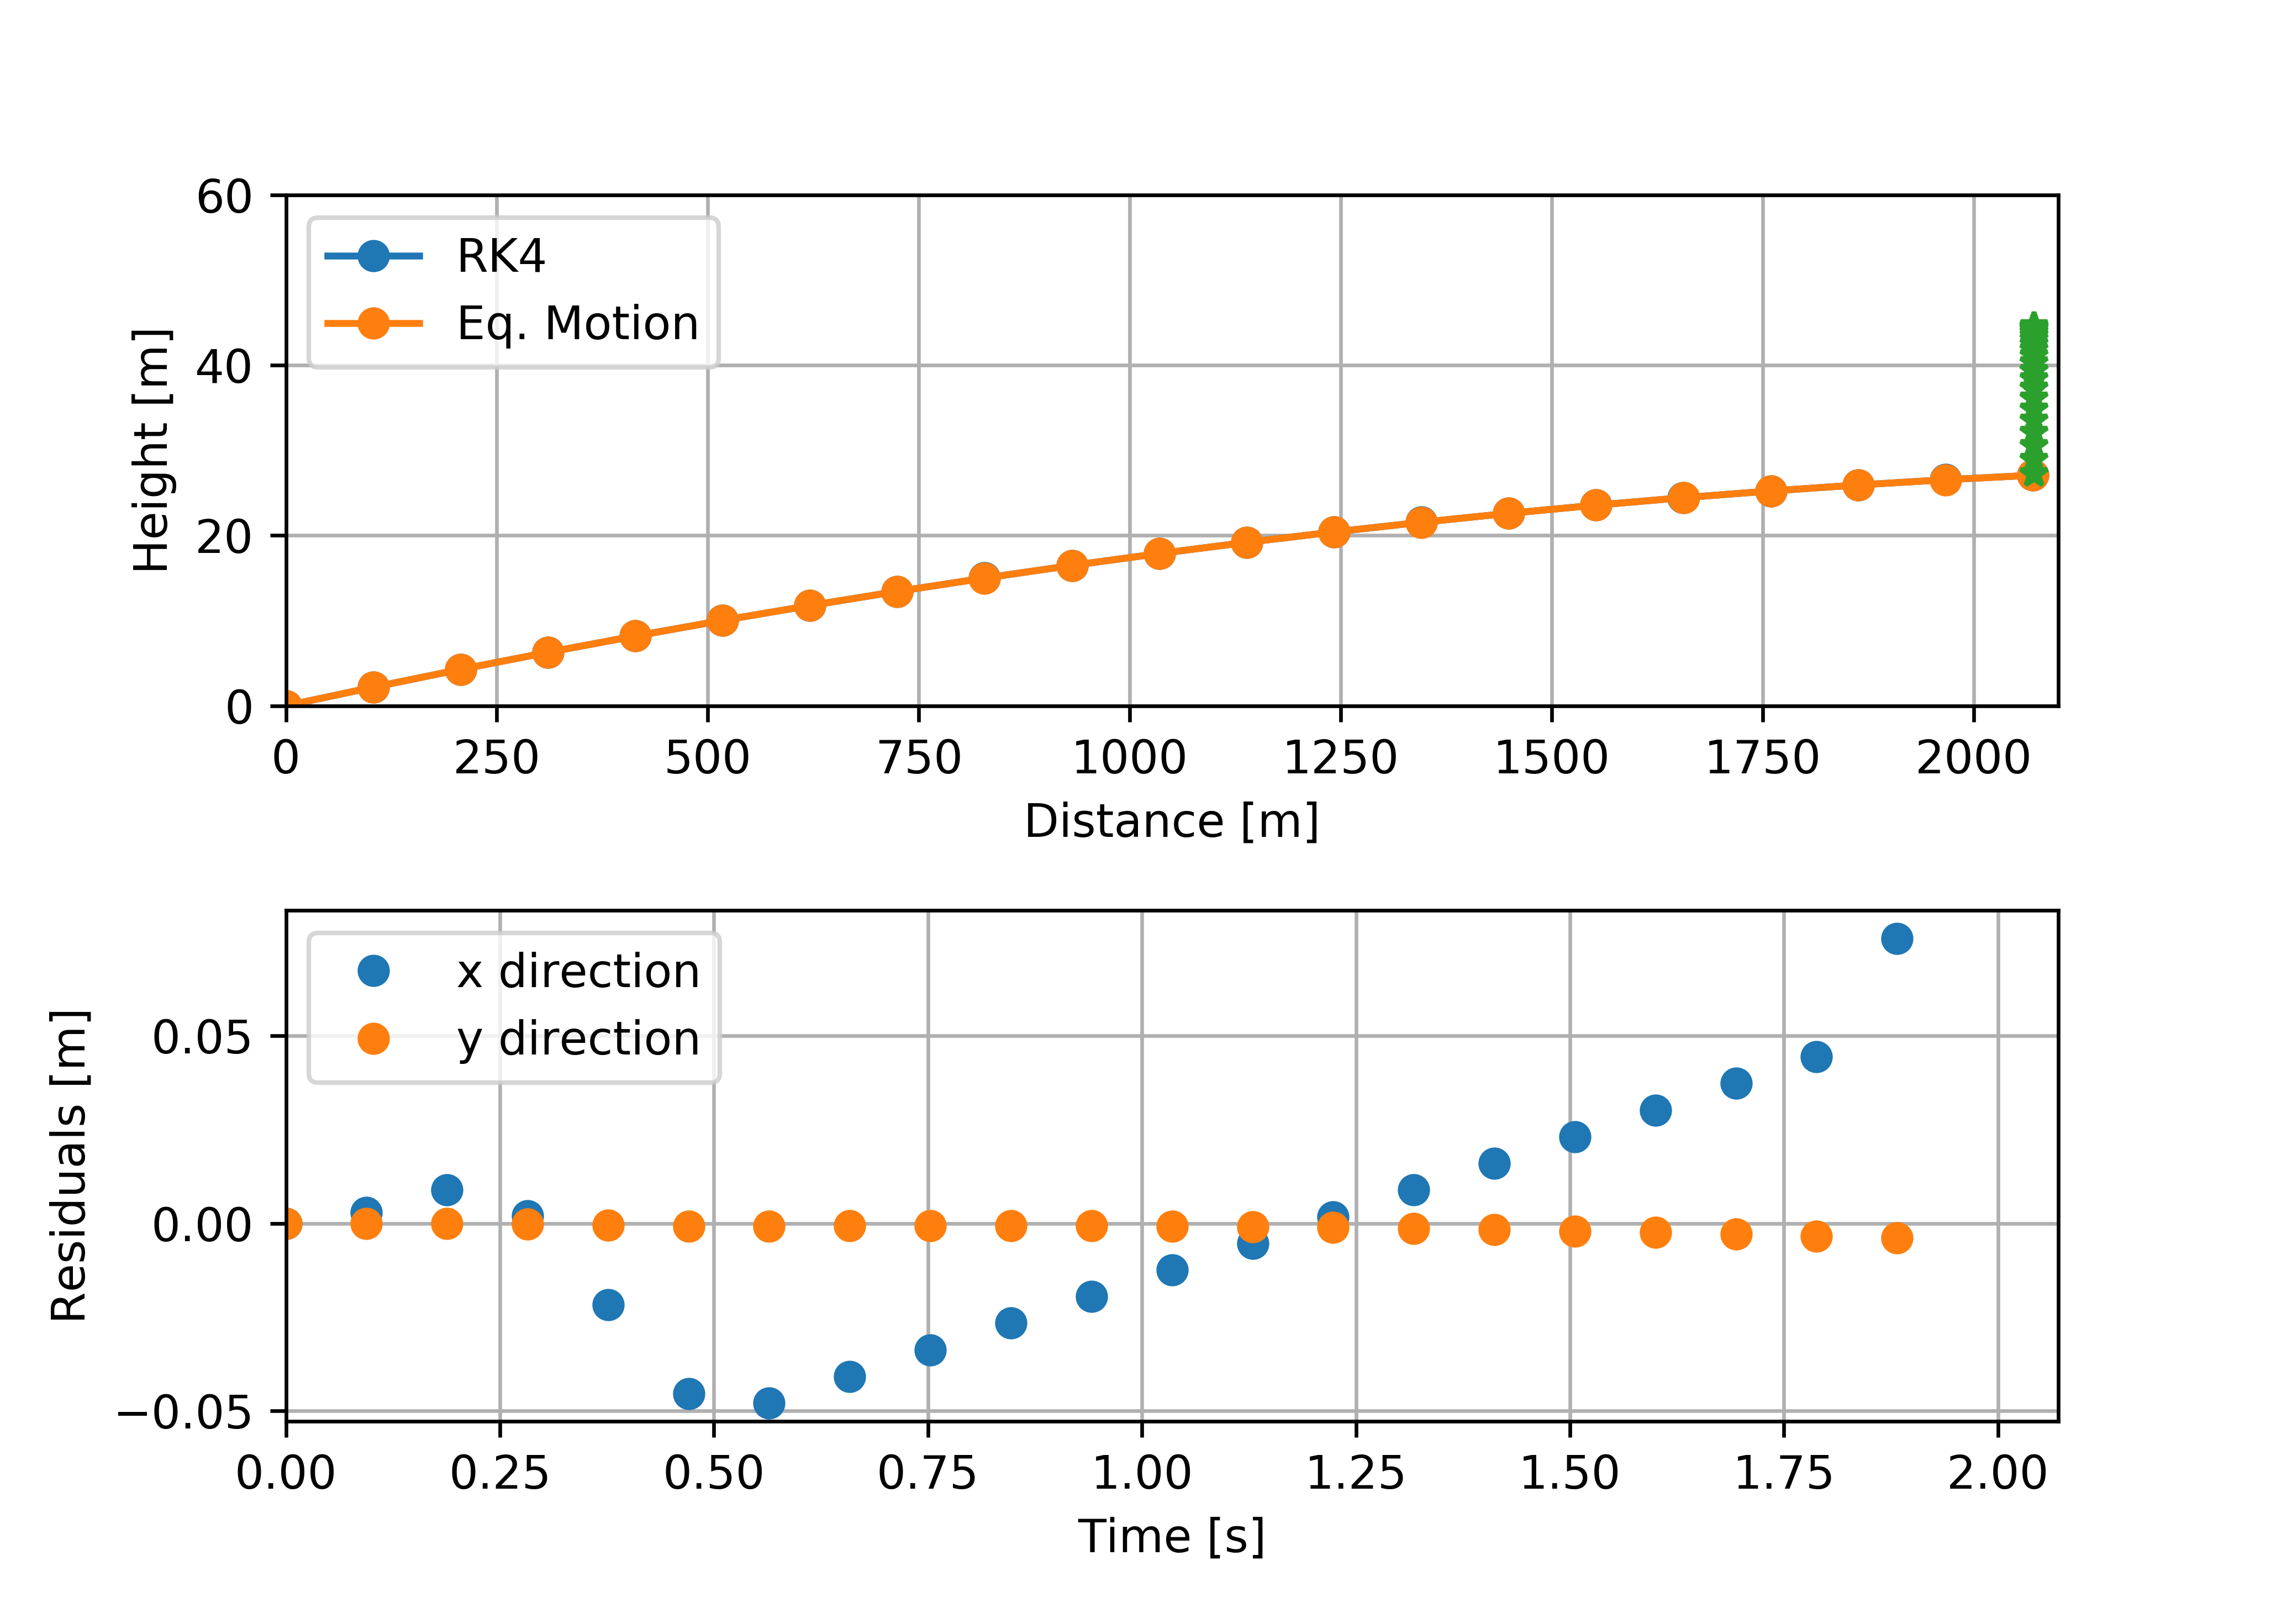
\includegraphics[width=.49\textwidth]{figures/a1-23x2071-4148y44-610104.png}
    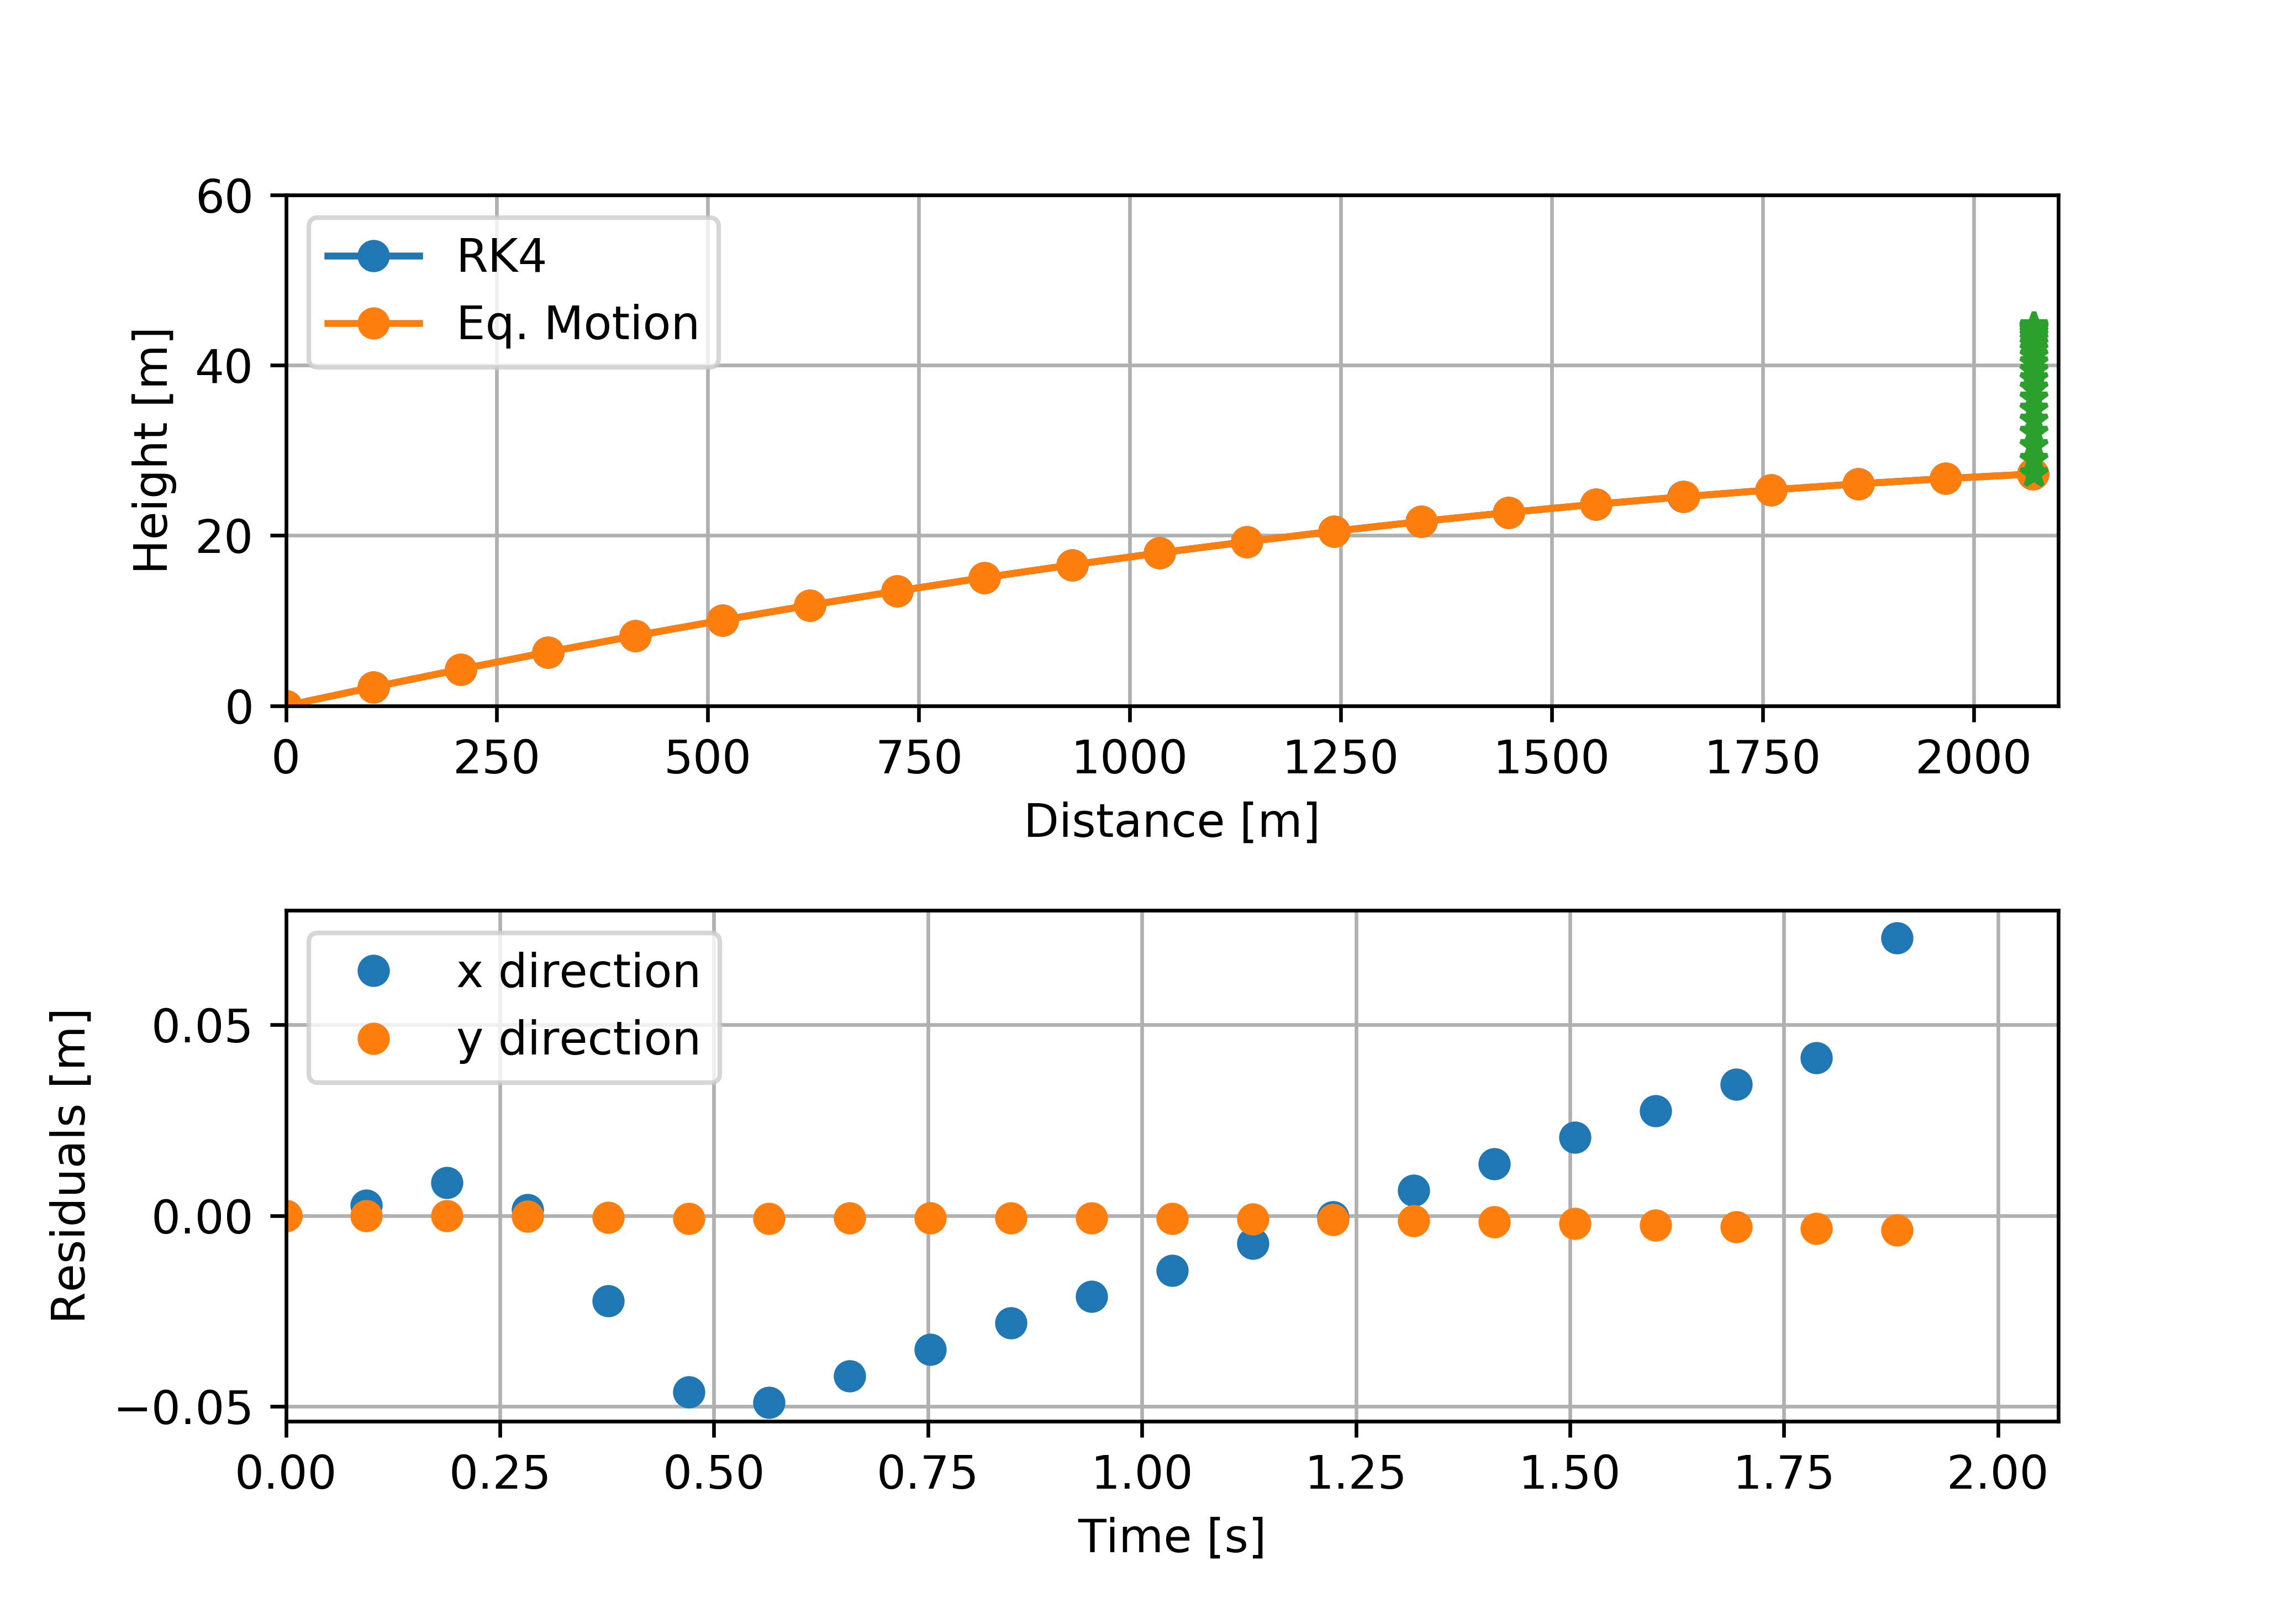
\includegraphics[width=.49\textwidth]{figures/a1-234x2071-4148y44-610104.png}
    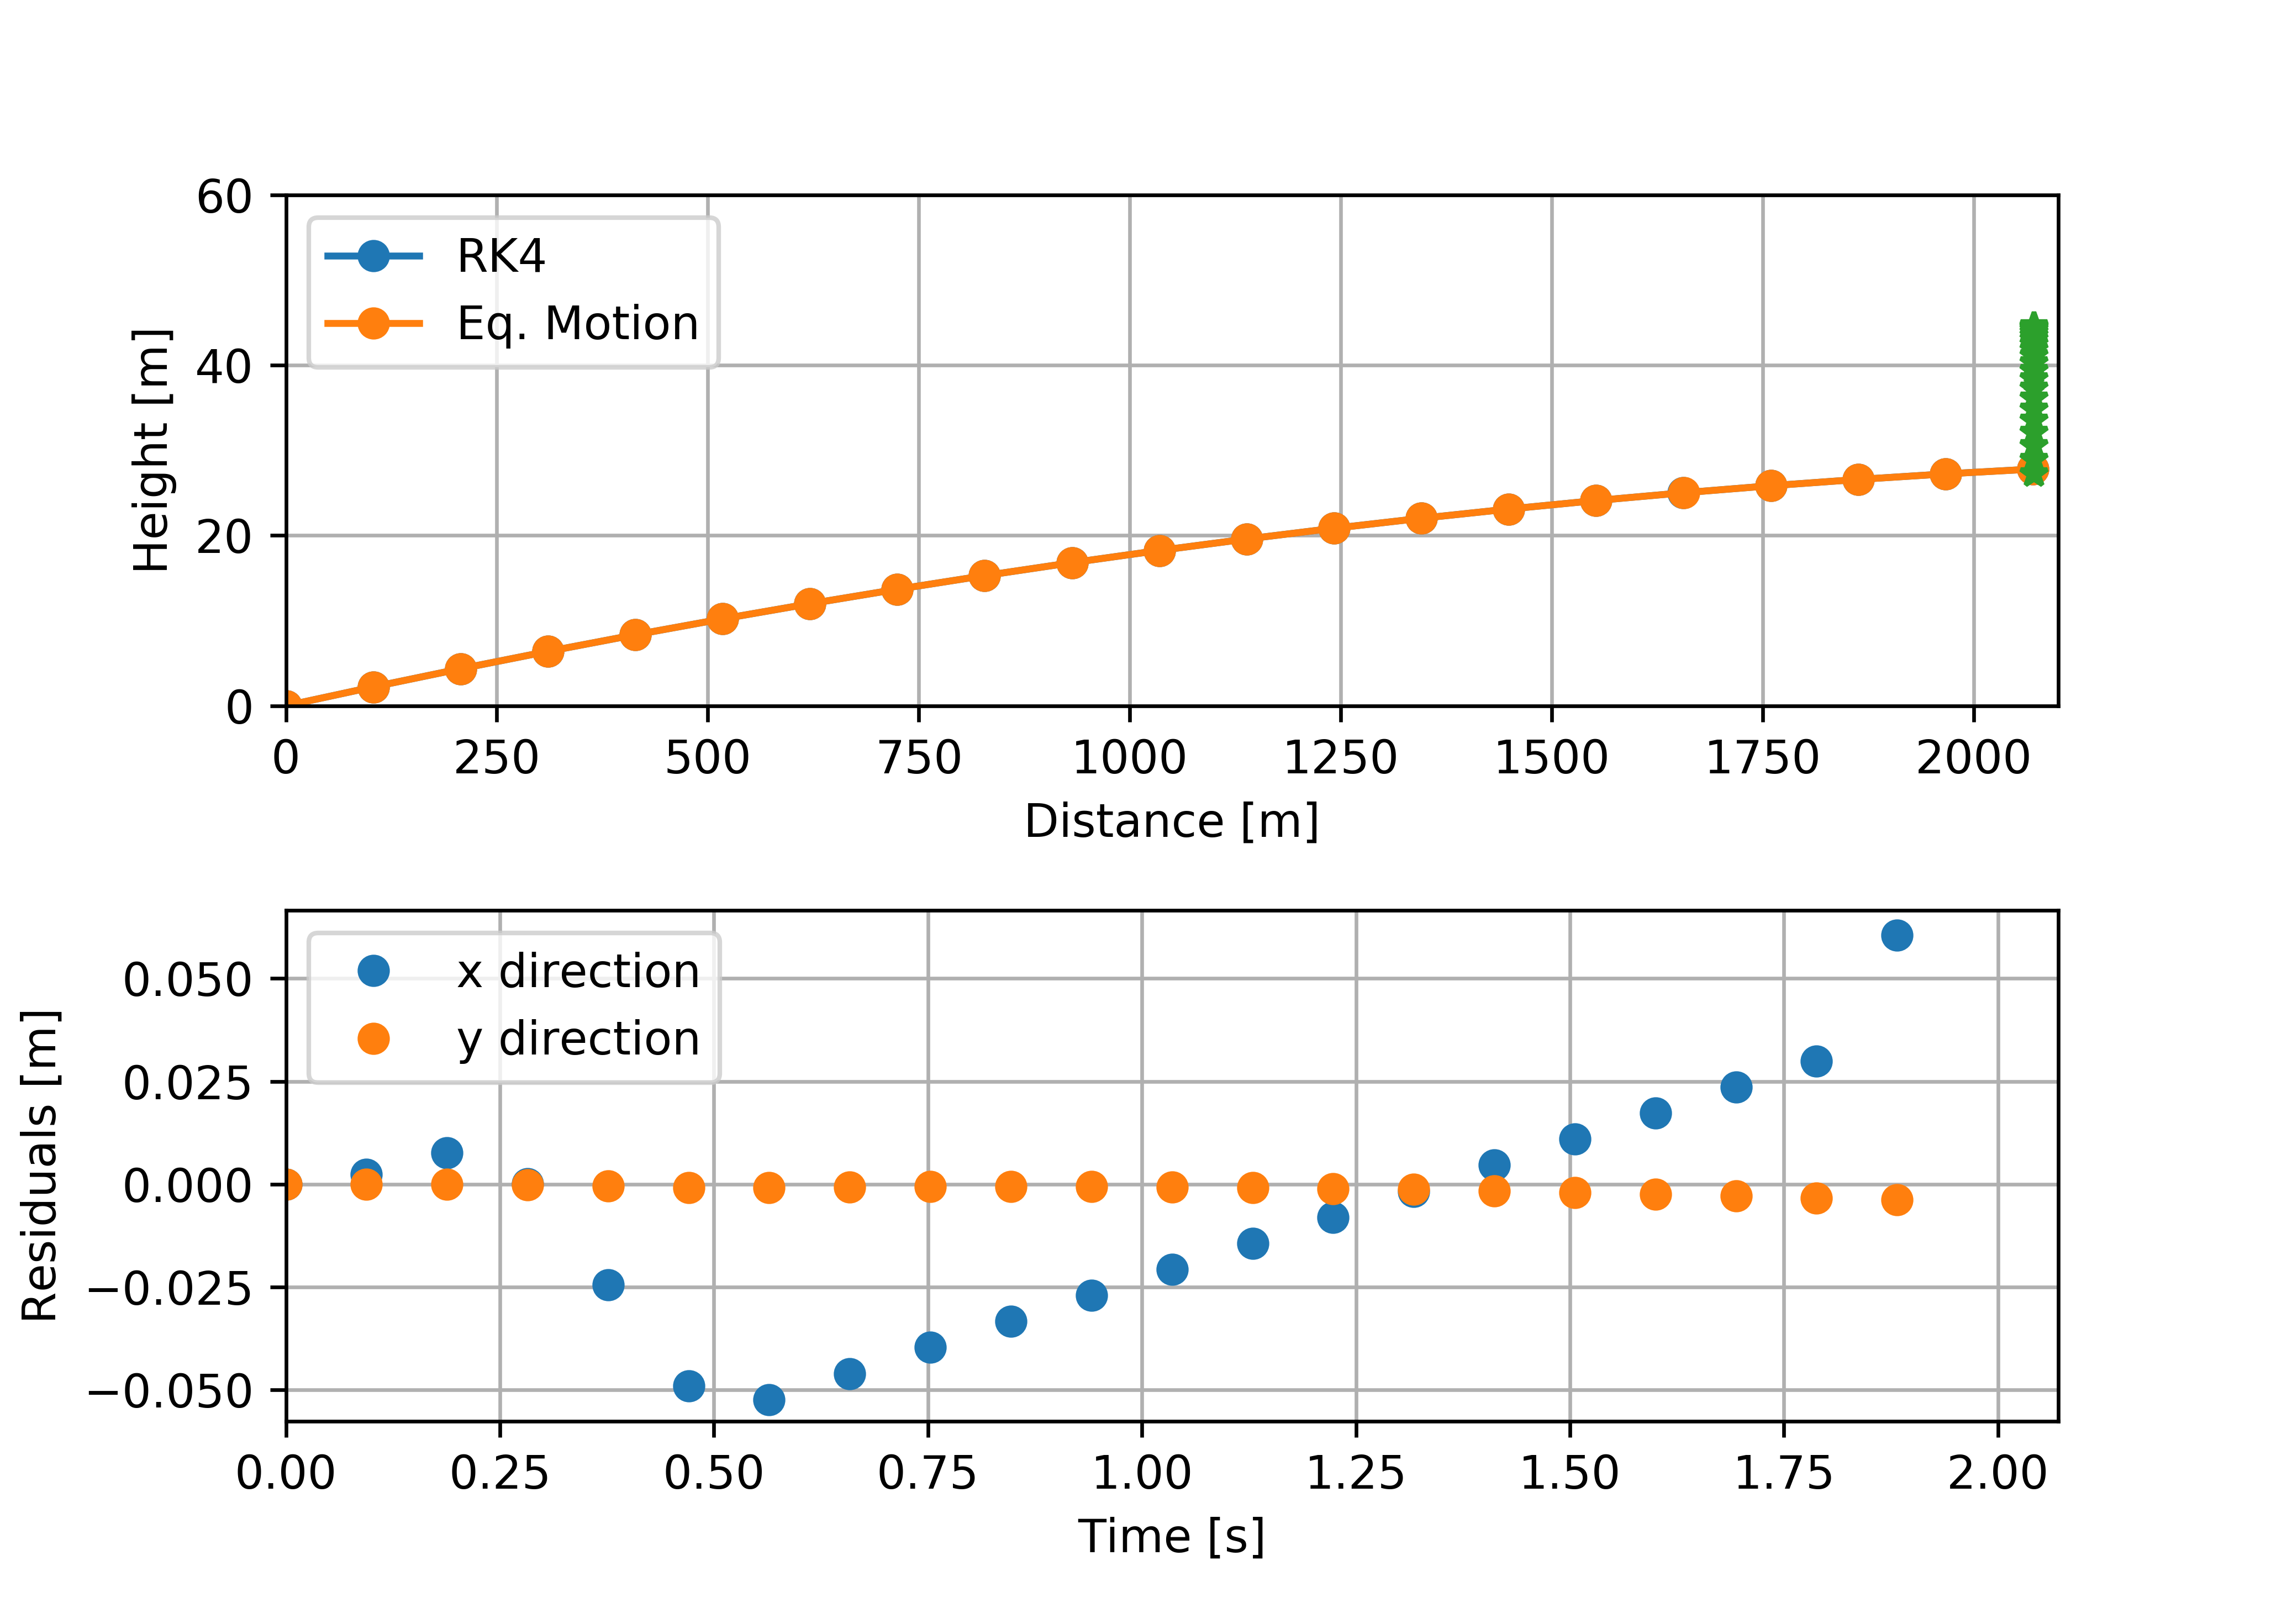
\includegraphics[width=.49\textwidth]{figures/a1-25x2071-4148y44-610104.png}
    \caption{Pairs of plots showing the trajectory followed by the golf ball using RK4 method and equations of motion as well as their residuals in x and y direction. All have distance of \SI{2071.41}{\m} and height of \SI{44.61}{\m}. Top Left: Angle of \ang{1.2},  Top Right: Angle of \ang{1.23}. Bottom Left: Angle of \ang{1.234}. This was a HIT. Bottom Right: Angle of \ang{1.25}.}
    \label{fig:diffAnglesSamePos}
\end{figure}











